\section{Spécifications fonctionnelles}

Le logiciel destiné au milieu médical, doit tout d'abord être en mesure de répondre à une interface simple et compréhensible par tous les utilisateurs. Dans notre cas, l'utilisateur peut être le thérapeute ou le patient. L'objectif étant d'optimiser au mieux l'interaction entre les différents objets et l'utilisateur \textit{via} des périphériques accessibles et ergonomiques. Par ailleurs, il faut aussi considérer que le thérapeute doit pouvoir accéder aux différentes options et le modifier afin de faciliter l'utilisation et l'intéraction dans la scène pour le patient.
\newline
Nous verrons dans une première partie les différents modes de navigation possibles, puis comment l'utilisateur peut selectionner et déplacer les objets présents dans la scène en fonction du mode d'apprentissage, et enfin toute la partie de gestion des options du logiciel pour le thérapeute.


\subsection{Scénarios d'utilisation}
Le cahier des charges qui nous a été fourni par le centre de Kerpape prévoit l'implémentation de différents scénarios d'utilisation centrés sur l'usage du domophone et que nous avons détaillés dans le premier rapport :
\begin{itemize}\renewcommand{\labelitemi}{$\bullet$}
\item Appel téléphonique normal
\item Appel \textit{via} l'interphone d'une personne venant fréquemment (un infirmier par exemple)
\item Appel \textit{via} l'interphone concernant une visite inattendue
\end{itemize}
Ces scénarios mettent en avant l'usage particulier qui peut être fait du téléphone et de la télévision (cf. \textsc{figure~\ref{domophone}}), car ceux-ci servent d'interphone, respectivement pour le son et l'image. Il faut donc que le téléphone, dans notre application, puisse recevoir des appels des deux types différents, mais aussi que la TV puisse recevoir le flux vidéo de l'interphone (en pratique dans les appartements tremplins, l'habitant doit se placer sur le canal 80 pour afficher la caméra de l'interphone).
\begin{figure}[h!]
	\begin{center}
  		\caption{Cas d'utilisation du domophone}
  		\label{domophone}
  		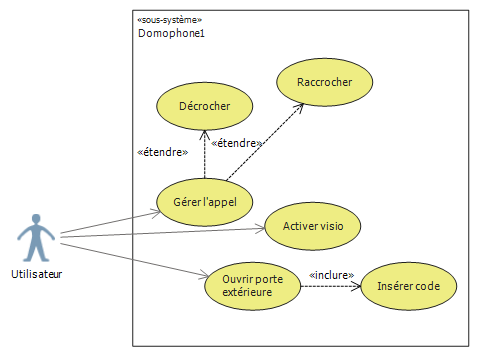
\includegraphics[width=\textwidth]{2-Specifications/img-utilisateur/use_case_diag.PNG}
  	\end{center}
\end{figure}

\subsection{Navigation}
Nous avons envisagé différents types de navigation au sein de l’environnement 3D, qui amèneront l’utilisateur à s’immerger et à interagir différemment avec la scène en fonction des périphériques utilisés.

\subsubsection{Exocentrée}
Avec un type de vue exocentré, l’utilisateur contrôle un avatar à la 3\up{ème} personne ce qui ne l’immergera pas totalement dans la scène. Cependant ceci peut permettre d'avoir une meilleure visualisation de la scène et de l'espace en 3D.
\newline
\textbf{Interface Souris - Clavier : }
L’utilisateur déplace son personnage à l’aide des touches du clavier. Il peut orienter la caméra l’aide de la souris. Pour entrer en interaction avec un objet il lui suffit de pointer l’objet avec la caméra et d’utiliser le clic gauche de la souris. L'orsqu'un objet est pointé il se met en légère sur-brillance.
Dans cette interface on définit les boutons suivants :
	\begin{itemize}\renewcommand{\labelitemi}{$\bullet$}
  				\item bouton d’action : clic gauche de la souris
				 \item bouton de retour : touche \em{escape} du clavier
  				\item  bouton 2\up{ème} action : clic droit de la souris
			\end{itemize}
Le thérapeute pourra modifier ces réglages s'il souhaite faire interagir l'utilisateur avec des boutons différents.
\newline


\textbf{Interface WiiMote - Nunchuk : }
Pour déplacer l’avatar, l’utilisateur s'appuiera sur le joystick du Nunchuk. Il peut orienter la caméra l’aide de la Wiimote. Pour entrer en interaction avec un objet il lui suffit de pointer l’objet avec la caméra et d’utiliser un des boutons de la Wiimote :
	\begin{itemize}\renewcommand{\labelitemi}{$\bullet$}
  				\item bouton d’action : bouton A de la WiiMote
				 \item bouton de retour :bouton Z du Nunchuk
  				\item  bouton 2\up{ème} action : bouton B de la WiiMote
			\end{itemize}

\subsubsection{Endocentrée}
En point de vue endocentré, l’utilisateur est plongé totalement dans l’environnement.
\newline
\textbf{Occulus Rift avec clavier-souis ou WiiMote-Nunchuk : }
De la même façon qu’en exocentré, l’utilisateur se déplacera et interagira avec la scène en utilisant l’interface clavier-souris ou WiiMote-Nunchuk. Cependant, on profite de ce point de vue immersif pour tirer profit des fonctionnalités de l’Occulus Rift.
Ce périphérique permettra la gestion de la caméra en orientant le champs de vision de l’utilisateur en fonction de ses mouvements de tête.
\newline
\textbf{Salle Immersia : }
La salle Immersia est une salle d’environnment 3D qui permet à l’utilisateur de s’intégrer totalement dans l’environnement virtuel. Ici une fois muni du capteur 3D dans l'espace, il pourra se déplacer totalement dans l’environnement.
Pour leur part les interactions seront effectuées grâce à une WiiMote.

\subsection{Sélection}

L'utilisateur, indépendamment du mode dans lequel il se trouve (Scénario ou déplacement libre), cf \ref{fig:modes}, peut interagir avec son environnement pour effectuer certaines actions ou tâches demandées par le thérapeute. Il peut donc actionner certains objet et voir les actions qu'il a effectuées dans son environnement. Cependant ces actions sont dépendantes du mode d'apprentissage dans lequel il se trouve. En effet, trois modes sont disponibles : Symbolique, Assisté et Autonome. Nous verrons dans cette partie les différentes actions qui se produise en fonction du mode d'apprentissage lorsque l'utilisateur interagit avec son milieu.

\begin{figure}[h]
  \centering
  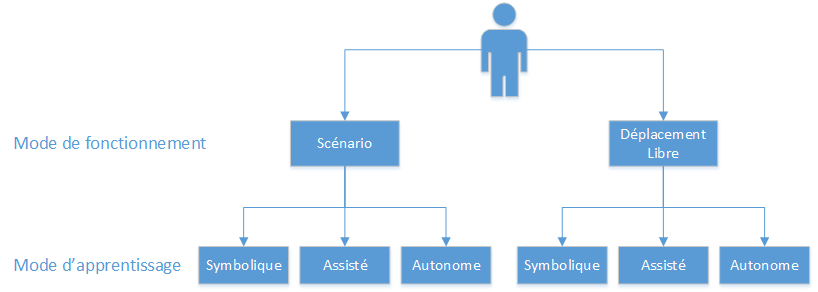
\includegraphics[width=1\textwidth]{2-Specifications/img-utilisateur/modes.png}
  \caption{\label{fig:modes} Choix des modes de fonctionnement et d'apprentissage}
\end{figure}


\subsubsection{Objets sélectionnables}

Avant de détailler le fonctionnement des différents modes, il est nécessaire d'expliciter les différents objets sélectionnables que l'on peut trouver dans l'appartement. On dénote dans la scène plusieurs objets qui permettent d'interagir avec le milieu :
\begin{itemize}
	\item Les interrupteurs pour les lumières, les portes internes et externes et les volets
	\item La télécommande qui comporte plusieurs boutons pour gérer notamment la télévision
	\item L'interphone qui permet de recevoir un appel
\end{itemize}

De même que précédemment, lorsque l'utilisateur pointe sur un objet, celui-ci se met en légère sur-brillance, il doit par la suite cliquer dessus pour pouvoir interagir avec. %Les interrupteurs, par un clic gauche (de la souris pas exemple), actionnent les différents éléments dans la pièce. %Pour la télécommande et l'interphone, le fonctionnement est un peu plus complexe : le premier clic permet d'avoir une vue zoomée sur l'objet et ainsi l'utilisateur peut selectionner le bouton qu'il souhaite actionner.


\subsubsection{Mode d'apprentissage : Symbolique}

La figure \ref{fig:MaquetteSymbolique} explique le fonctionnement lorsque l'utilisateur interagit avec un objet dans le mode symbolique. Elle est accompagné d'un diagramme d'activité (figure \ref{fig:CasUsageSymbolique}) pour une meilleur compréhension.
\newline
Lorsque l'utilisateur est dans un scénario ou dans un didacticiel, l'objet se met en sur-brillance dans la scène. L'utilisateur se déplace jusqu'à l'objet et rentre dans dans une vue symbolique qui lui explique le fonctionnement de l'objet. Dans notre exemple ici, pour l'ouverture d'une porte, l'utilisateur reçoit les consignes pour ouvrir la porte. Par exemple : « Le bouton du haut permet de fermer la porte, celui du bas de l'ouvrir. Si vous souhaitez ouvrir la porte il faut donc appuyer sur le bouton du bas ». Les consignes sont liées à des indications fléchées qui aident à la compréhension. Par la suite, l'utilisateur peut actionner le bouton. Cette action lance une animation qui montre de manière symbolique l'ouverture de la porte.
\newline
En fonction du didacticiel plusieurs apprentissages peuvent se produire à la suite, ouverture de la porte puis fermeture par exemple. Si l'utilisateur ne souhaite plus interagir avec l'objet il peut a tout moment quitter la vue symbolique avec la touche «esc».

\begin{figure}[h]
\centering
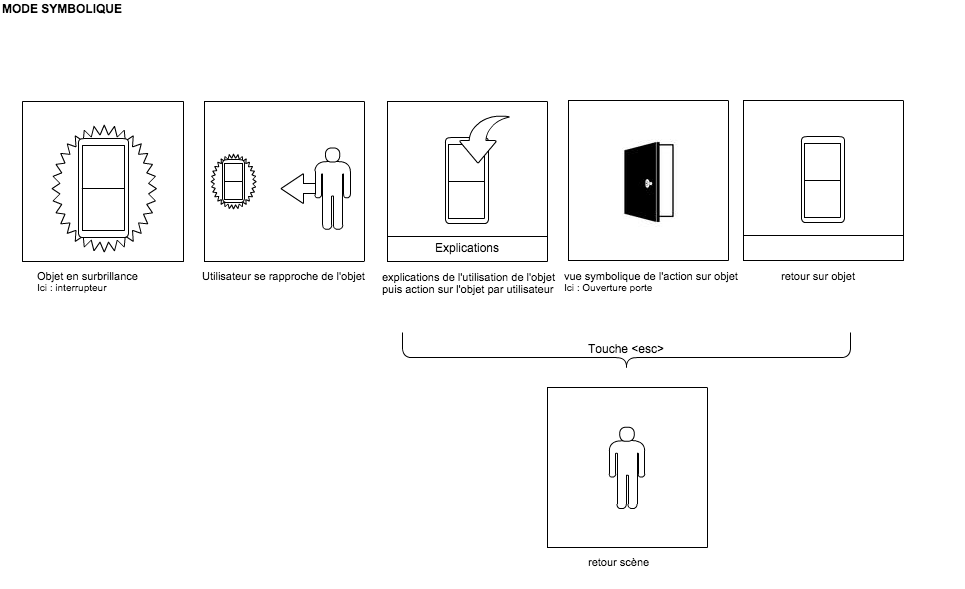
\includegraphics[width=1\textwidth]{2-Specifications/img-utilisateur/symbolique.png}
\caption{\label{fig:MaquetteSymbolique} Manipulation d'objets dans le mode Symbolique }
\end{figure}
\begin{figure}[h]
\centering
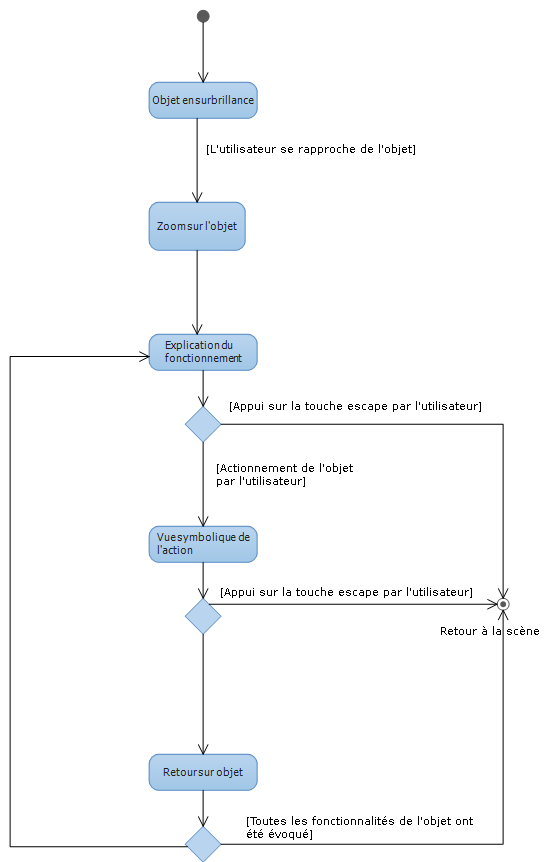
\includegraphics[width=1\textwidth]{2-Specifications/img-utilisateur/activite-symbolique.png}
\caption{\label{fig:CasUsageSymbolique} Diagramme d'activité : Manipulation d'objets dans le mode Symbolique }
\end{figure}
\FloatBarrier


\subsubsection{Mode d'apprentissage : Assisté}

Après un apprentissage Symbolique, l'ergothérapeute peut décider de passer à un apprentissage Assisté. Dans ce dernier, l'utilisateur doit entreprendre plus d'actions que précédemment pour interagir avec l'objet. Comme précédemment, si l'utilisateur est dans un scénario ou didacticiel, l'objet se met en sur-brillance. L'utilisateur se rapproche alors et doit cliquer sur l'objet. Si celui-ci comporte plusieurs boutons (télécommande par exemple), une vue «zoomée» de l'objet apparaît et l'utilisateur peut cliquer sur le bouton qu'il doit actionner. Une fois le bouton cliqué, une fenêtre apparaît et montre en 3d l'action qui a été effectué.
\newline
Les figures \ref{fig:MaquetteAssiste} et \ref{fig:CasUsageAssiste} reprennent le fonctionnement de ce mode.

\begin{figure}[h]
\centering
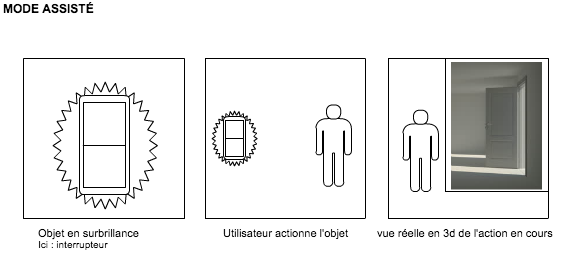
\includegraphics[width=1\textwidth]{2-Specifications/img-utilisateur/assiste.png}
\caption{\label{fig:MaquetteAssiste} Manipulation d'objets dans le mode Assisté }
\end{figure}
\begin{figure}[h]
\centering
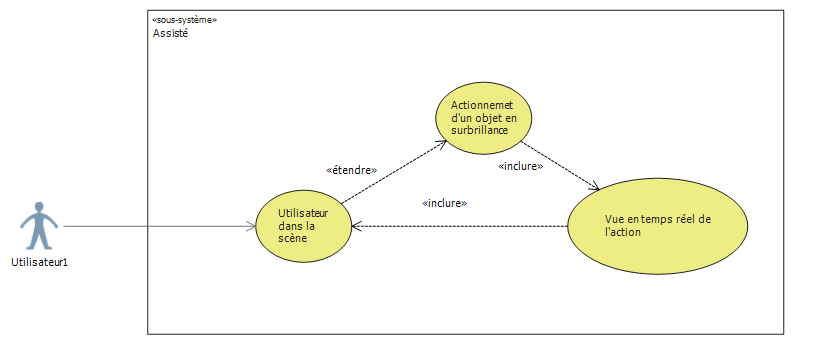
\includegraphics[width=1\textwidth]{2-Specifications/img-utilisateur/cas-usage-assiste.png}
\caption{\label{fig:CasUsageAssiste} Diagramme de cas d'usage : Manipulation d'objets dans le mode Assisté }
\end{figure}
\FloatBarrier


\subsubsection{Mode d'apprentissage : Autonome}

Le mode autonome ne donne plus aucune indication à l'utilisateur. L'objet n'est plus en sur-brillance dans le cas de scénarios ou didacticiels. Il doit aller actionner lui même l'objet comme précédemment et se rendre compte en se déplaçant dans la scène si son action est bien la bonne.
\newline
Les figures \ref{fig:MaquetteAutonome} et \ref{fig:CasUsageAutonome} reprennent le fonctionnement de ce mode.

\begin{figure}[h]
\centering
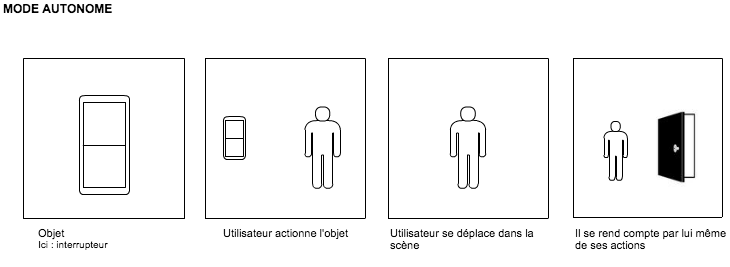
\includegraphics[width=1\textwidth]{2-Specifications/img-utilisateur/autonome.png}
\caption{\label{fig:MaquetteAutonome} Manipulation d'objets dans le mode Autonome }
\end{figure}
\begin{figure}[h]
\centering
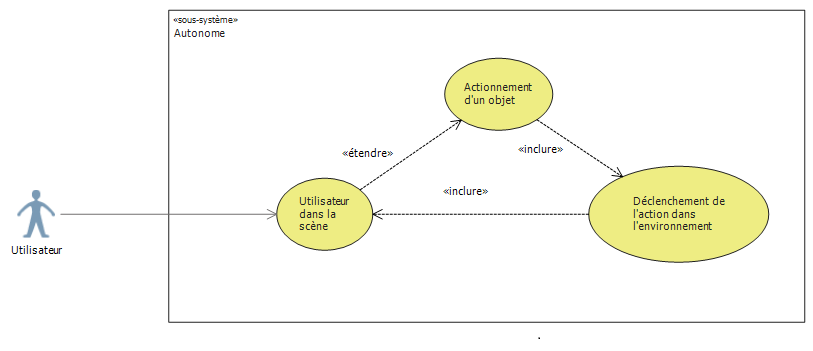
\includegraphics[width=1\textwidth]{2-Specifications/img-utilisateur/cas-usage-autonome.png}
\caption{\label{fig:CasUsageAutonome} Diagramme de cas d'usage : Manipulation d'objets dans le mode Autonome }
\end{figure}
\FloatBarrier



\subsection{Manipulation}
Dans l’appartement, l’utilisateur est amener à manipuler différents types d’objet : un interphone, des interrupteurs et une télécommande

\subsubsection{Manipulation de l’interphone }
Une fois l’interphone sélectionné par l’utilisateur (par l’appui sur une touche ou automatiquement en fonction du mode d’apprentissage), ce dernier aura un affichage de l’appareil. Il pourra ensuite l’utiliser en appuyant sur ses touches grâce au pointeur de la souris ou de la Wiimote, (qui ne gère plus la caméra lors de ce type d’événement) et l’appui sur la touche d’action. La manipulation de l’interphone se termine lorsque l’utilisateur appuie sur la touche de retour ou qu’il a correctement terminé l’action à effectuer du scénario. L’utilisateur bascule alors sur l’appartement.

\subsubsection{Manipulation d’un interrupteur}
L’utilisateur s’approche de l’interrupteur, et l’actionne grâce à l’appui sur le bouton d’action. En fonction du mode d’apprentissage, il y a affichage centré ou non sur l’objet. Le retour à la scène se fait automatiquement une fois l’action terminé ou par l’appui sur la touche de retour.

\subsubsection{Manipulation de la télécommande}
Si l’utilisateur n’a pas encore pris la télécommande il peut aller la chercher dans l’environnement. Une fois qu’elle est sélectionnée, il peut l’utiliser grâce au pointeur de la souris ou de la WiiMote et à l’appui sur le bouton d’action. A tout moment, il peut la reposer grâce au bouton de retour. Ses actions terminées, il peut la reposer ou la garder avec lui en appuyant sur le bouton de deuxième action.

\subsection{Contrôle d’application}
\subsubsection{Administrateur}
Pour le contrôle de l'application, le thérapeute sera considéré comme administrateur de l'application. Il a accès à
tous les paramètres de configurations et choisir les différents modes (scénarios,didacticiels,déplacement libre) pour l'Utilisateur.
\newline
Les figures \ref{fig:Menu} et \ref{fig:CasUsageMenu} reprennent le fonctionnement global de l'interface. Ainsi sur le menu principal, le thérapeute peut choisir entre les Didacticiels, les Scénarios, se déplacer librement ou les Options.
\newline
Les Options permettent de configurer le choix des touches ainsi que certains paramètres plus personnalisés pour l'utilisateur. On peut ainsi charger/sauvegarder un fichier utilisateur avec les configurations des touches, taille de personnage, télécommande personnalisée, qui ont été au préalable déjà configurés.

On peut aussi choisir, si la configuration le permet (Clavier/Souris, Occulus, Salle Immersia), le mode de Navigation (endocendré ou exocentré).
\newline
Lorsque les configurations de bases ont été effectuées, le thérapeute peut alors choisir un des différents modes. Si l'on choisit un Scénario ou un Didacticiel, le mode d'apprentissage (Symbolique, Assisté, Autonome) sera demandé. Dans le cas du déplacement libre, le mode d'apprentissage est Autonome par défaut. Le mode d'apprentissage peut-être ultérieurement changé dans le menu d'option de la scène si le thérapeute le souhaite.
\newline

\begin{figure}[h]
\centering
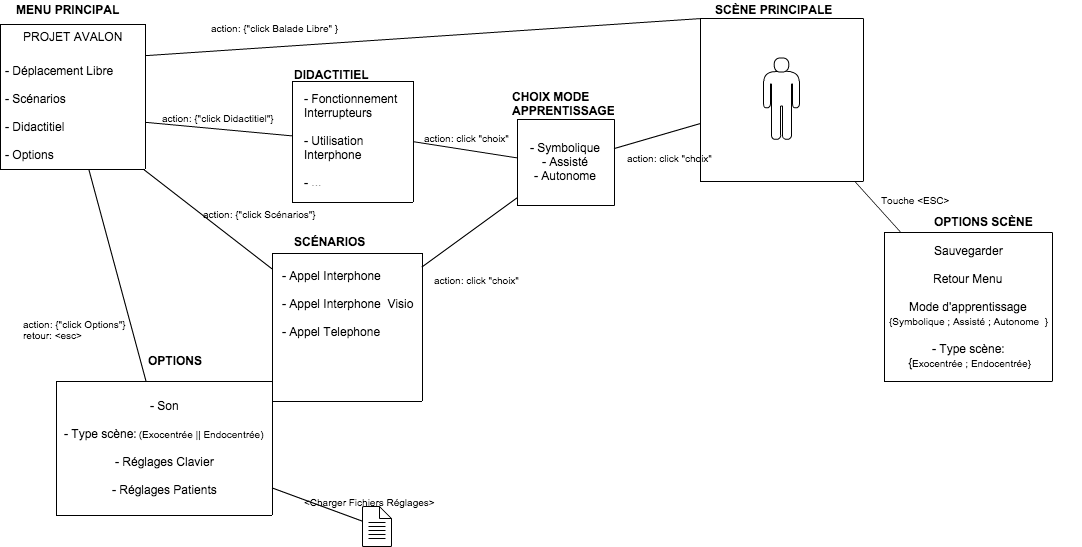
\includegraphics[width=1\textwidth]{2-Specifications/img-utilisateur/menu.png}
\caption{\label{fig:Menu} Menu principal et configurations environnement }
\end{figure}
\begin{figure}[h]
\centering
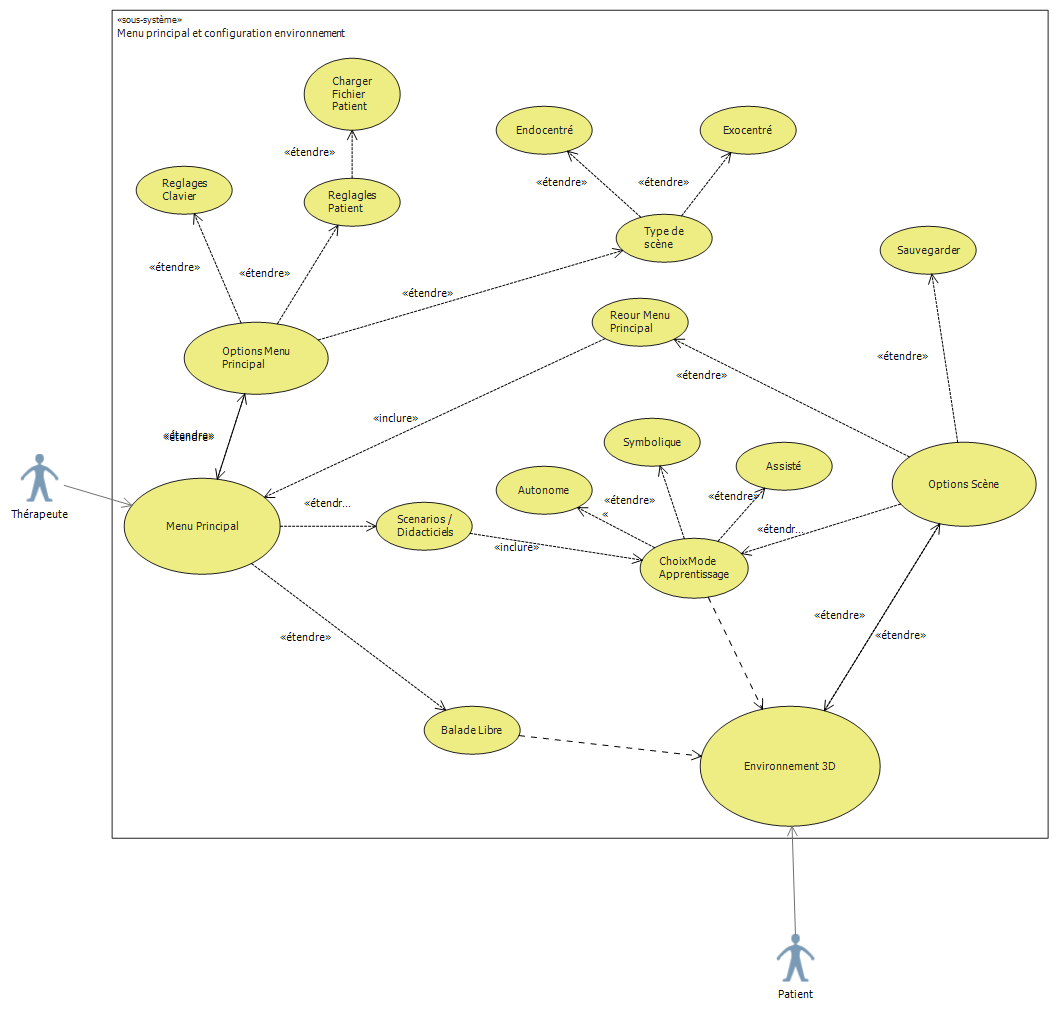
\includegraphics[width=1\textwidth]{2-Specifications/img-utilisateur/cas-usage-menu.png}
\caption{\label{fig:CasUsageMenu} Diagramme de cas d'usage : Menu principal et configurations environnement }
\end{figure}
\FloatBarrier

<<<<<<< HEAD
\subsubsection{Salle immersive}

il ne faut pas hésiter à dire que c’est un projet important avec un réel enjeu.
Il a plusieurs raisons à utiliser des plateformes telles que Immersia et µRV : la solution du casque est exploratoire pour Kerpape,
mais on sait déjà qu’elle présente quelques risques  : équipement assez lourd qui peut poser problème pour les patients, perte des repères de son propre corps (on ne voit plus ses mains)… 
Les plateformes de RV Immersia, minImmersia et µRV permettent d’évaluer des formes d’interactions plus naturelles. 
D’autre part, le fait d’être capable d’utiliser différents types de plateformes permettra de laisser le projet ouvert par la suite à d’autres utilisations dans le domaine de la rééducation fonctionnelle. 
Enfin, ces plateformes sont des vitrines du département info et du labo, elles permettront donc de donner plus de visibilité à ce projet très important.


La salle immersive représente l'équipement de RV le plus complet dont nous puissions profiter et est donc une perspective de plate-forme très intéressante pour notre application.
\begin{wrapfigure}{l}{0mm}
	\centering
	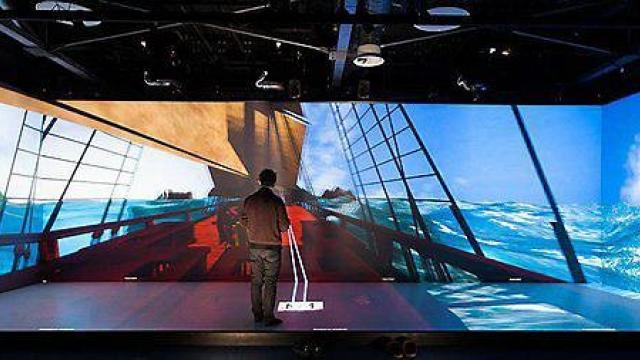
\includegraphics[scale=0.5]{2-Specifications/img-utilisateur/immersia.jpg}
\end{wrapfigure}
C'est l'option qui nous permettra les interactions les plus naturelles, car l'utilisateur se trouvera dans une projection à l'échelle 1:1 de l'appartement, équipé de lunettes 3D et de capteurs qui permettent de suivre la position des mains de l'utilisateur. \newline
L'utilisation d'une plateforme de ce type permet d'éviter les quelques risques liée à l'utilisation de périphériques portés par l'utilisateur
Bien que Kerpape n'en dipose pas et n'ait pas la possibilité d'en utiliser une, l'implémentation du projet Avalon dans une salle immersive reste donc un objectif que nous souhaitons réaliser.
=======

\subsubsection{Utilisateur}
Finalement, l'utilisateur n'a accès qu'à la scène. Il peut ainsi interagir avec les objets en fonction du Scénario et du mode d'Apprentissage. Il n'a pas à se soucier des configurations. En parallèle le thérapeute peut vérifier si les actions sont effectués comme prévu et réajuster le mode d'apprentissage ou changer de type de vue si nécessaire.
>>>>>>> 7ed213898782ba1d884805ac5c0f3f7fdb8328f8
